%% Define title of slide deck

\newcommand\CourseTopic{Advanced R: Visualization and Programming}
\newcommand\CourseTopicShort{Advanced R}
\newcommand\CourseNumber{3}

\newcommand\CourseDate{\today}
\newcommand\CourseInstitute{ETH Zurich}
\newcommand\CourseAbbreviation{OR}
\newcommand\CourseTitle{Operations Research in R}
\newcommand\CourseAuthor{Stefan Feuerriegel}

\newcommand{\CourseQuiz}{Visit webpage with course quiz.}
\newif\ifQuizSolution\QuizSolutionfalse

\PassOptionsToPackage{table,dvipsnames}{xcolor}
\documentclass[%
  final,
  11pt, 
  show notes, % enables Notes
  t, % Place text of slides at the (vertical) top of the slides
  fleqn, % equations are centered
]{beamer} 

\usepackage{booktabs}

\newcommand\const{\mathsf{const.}}
\newcommand\rp{^{-1}}
\newcommand\rps{^{-2}}
\newcommand\rpc{^{-3}}

\newcommand\transpose{^T} %{^\top}
\newcommand\rptranspose{^{-T}} %^{^{-\top}}
\newcommand\pseudoinverse{^{+}}

\newcommand\define{:=} % :=, \ensuremath{\mathrel{\stackrel{\mathsf{def}}{=}}}
\newcommand\ldefine{=:}
\newcommand{\setsep}{\, | \,}

\newcommand{\correspond}{\mathrel{\widehat{=}}}

\newcommand{\norm}[1]{\left\Vert #1 \right\Vert}
\newcommand{\floor}[1]{\left\lfloor #1 \right\rfloor}
\newcommand{\ceil}[1]{\left\lceil #1 \right\rceil}

\newcommand{\vecval}[1]{\bm{#1}}
\newcommand{\matval}[1]{#1}

\newcommand{\sspace}{\quad}
\newcommand{\wspace}{\qquad}

\newcommand{\sand}{\sspace\text{and}\sspace}
\newcommand{\wand}{\wspace\text{and}\wspace}
\newcommand{\for}{\text{for }}

\newcommand{\R}{\mathbb{R}}
\newcommand{\N}{\mathbb{N}}

\newcommand{\unitvec}[2]{{\vecval{u}_{#1}}}
\newcommand{\identitymat}[1]{\matval{\mathup{I}}_{#1,#1}}
\newcommand{\permutemat}{\matval{\Pi}}
\newcommand{\zerovec}[1]{\vecval{0}_{#1}}
\newcommand{\zeromat}[2]{\matval{0}_{#1,#2}}

\newcommand{\fulfill}{\stackrel{!}{=}}
\newcommand{\inlineortho}{\bot}
\newcommand{\ortho}{\,\, \inlineortho \,\,}
\newcommand{\iszero}[1]{\underbrace{#1}_{=0}}

\newcommand{\vecsize}[1]{\in\R^{#1}}
\newcommand{\matsize}[2]{\in\R^{#1 \times #2}}

\newcommand{\concatmat}[1]{\Concat{#1}}
\newcommand{\concatvec}[1]{\left[#1\right]}
\newcommand{\concatmatsep}{\, | \,}
%\newcommand{\lincomb}[1]{\left\langle #1 \right\rangle}
\newcommand{\lincomb}[1]{\linearspan{#1}}
%\newcommand{\vecprod}[2]{\left( #1, #2 \right)}
\newcommand{\vecprod}[2]{\left\langle #1, #2 \right\rangle}

\newcommand{\abs}[1]{\left\lvert #1 \right\rvert}
\newcommand{\sign}[1]{\mathup{sign}\left( #1 \right)}
%\newcommand{\ssign}{\mathsf{sign}}
\newcommand{\diag}{\operatorname{diag}}
%\renewcommand\Re[1][]{\mathsf{Re}\,#1}
%\renewcommand\Im[1][]{\mathsf{Im}\,#1}

\newcommand{\vvector}[2]{\left[\begin{array}{c} #1 \\ #2 \end{array} \right]}
\newcommand{\vvvector}[3]{\left[\begin{array}{c} #1 \\ #2 \\ #3 \end{array} \right]}

\newcommand{\intervaloo}[2]{\left(#1,#2\right)}
\newcommand{\intervaloc}[2]{\left(#1,#2\right]}
\newcommand{\intervalco}[2]{\left[#1,#2\right)}
\newcommand{\intervalcc}[2]{\left[#1,#2\right]}

\newenvironment{mmatrix}{\begin{bmatrix}}{\end{bmatrix}}

\newcommand{\Oh}[1]{\mathsf{O}\left(#1\right)}

\newcommand{\e}[1]{\mathup{e}^{#1}}

\newcommand{\dd}{\mathop{}\!\mathsf{d}}
\newcommand{\Laplace}{\Updelta}

\newcommand\op[1]{{\hat{\mathsf{#1}}}}  % Operator

\newcommand\imaginary{\mathup{i}}

% use together with long limits in \sum, \prod, etc
% from mathmode, p. 63
  \def\clap#1{\hbox to 0pt{\hss#1\hss}}
  \def\mathclap{\mathpalette\mathclapinternal}
  \def\mathclapinternal#1#2{%
    \clap{$\mathsurround=0pt#1{#2}$}
  }

\newcommand\ie{i.\,e.\xspace}
\newcommand\eg{e.\,g.\xspace}
\newcommand\etc{etc.\xspace}
\newcommand\cf{cf.\xspace}

%% from: http://tex.stackexchange.com/questions/2441/how-to-add-a-forced-line-break-inside-a-table-cell
\newcommand{\mcell}[2][c]{%
  \begin{tabular}[c]{@{}#1@{}}#2\end{tabular}}
\newcommand{\mcellt}[2][c]{%
  \begin{tabular}[t]{@{}#1@{}}#2\end{tabular}}

\newcommand{\stackedcell}[2][c]{%
  \begin{tabular}[#1]{@{}c@{}}#2\end{tabular}}

<<setup, include=FALSE>>=
# change default language to display error messages in English
Sys.setenv(LANGUAGE = "en")

# smaller font size for chunks
library(knitr)
opts_chunk$set(size = "footnotesize", fig.width = 3, fig.height = 3)
@

<<setup_custom, include=FALSE>>=
opts_chunk$set(fig.width = 6, fig.height = 3, dpi = 50, out.width = ".9\\textwidth")
@

\begin{document}

  \begin{frame}%[plain]
  \titlepage
\end{frame}
  
\begin{frame}
  \frametitle{Today's Lecture}
\vfill
\begin{block}{Objectives}
\begin{enumerate}
\item Visualizing data in R graphically as points, lines, contours or areas
\item Understanding the programming concepts of if-conditions and loops
\item Implementing simple functions in R
\item Measuring execution time
\end{enumerate}
\end{block}
\vfill
\end{frame}
  
  % \section[Contents]{}

\begin{frame}<beamer>%[allowframebreaks]
  \frametitle{Outline}
  \tableofcontents[%
%     currentsection, % causes all sections but the current to be shown in a semi-transparent way.
%     currentsubsection, % causes all subsections but the current subsection in the current section to ...
%     hideallsubsections, % causes all subsections to be hidden.
%     hideothersubsections, % causes the subsections of sections other than the current one to be hidden.
%     part=, % part number causes the table of contents of part part number to be shown
%    pausesections, % causes a \pause command to be issued before each section. This is useful if you
%     pausesubsections, %  causes a \pause command to be issued before each subsection.
%     sections={ overlay specification },
%      sectionstyle=show/shaded,
      subsectionstyle=hide
  ]
\end{frame}

\section{Visualization}

\begin{frame}[fragile]
  \frametitle{Point Plot}
\begin{itemize}
\item Creating simple point plots (also named scatter plots) via \verb@plot(...)@
\item Relies upon vectors denoting the x-axis and y-axis locations
\item Various options can be added to change appearance
\end{itemize}

<<pointplot,out.width='\\textwidth',dpi=50,echo=-1,tidy=FALSE,size='scriptsize'>>=
setwd("../Datasets/")
d <- read.csv("persons.csv", header=TRUE, sep=",", 
              stringsAsFactors=FALSE)
plot(d$height, d$age)
@
\end{frame}

\begin{frame}[fragile]
  \frametitle{Adding Title, Labels and Annotations}
\begin{itemize}
\item Title is added through additional parameter \verb@main@
\item Axis labels are set via \verb@xlab@ and \verb@ylab@
\item Annotations next to points with \verb@text(...)@
%\item Their position is specified with \verb@pos=2@
\end{itemize}
<<pointplot-with-labels,out.width='.8\\textwidth',fig.keep='last',dpi=50,tidy=FALSE>>=
plot(d$height, d$age, 
     main="Title",              # title for the plot 
     xlab="Height", ylab="Age") # labels for x and y axis
text(d$height, d$age, d$name) # d$name are annotations
@
\end{frame}

\begin{frame}[fragile]
  \frametitle{Line Plot}
Generate line plot using the additional option \verb@type="l"@
<<lineplot,out.width='\\textwidth',fig.keep='last',dpi=50>>=
x <- seq(0, 4, 0.01)
plot(x, x*x, type="l")
@
\end{frame}

\begin{frame}[fragile]
  \frametitle{Exercise: Plotting}
<<exercise_plotting_x,eval=FALSE>>=
x <- seq(-1, +1, 0.01)
@
<<,include=FALSE>>=
<<exercise_plotting_x>>
@
<<exercise_plotting,out.width='.5\\textwidth',fig.keep='last',dpi=50,echo=FALSE>>=
plot(x, abs(x), type="l", ylab="", xlab="")
@
\begin{exampleblock}{Question}
\begin{itemize}
\item How would you reproduce the above plot?
\begin{itemize}
\item \verb@plot(x, kink(x), type="l", main="")@
\item \verb@plot(x, kink(x), type="l", lab="")@
\item \verb@plot(x, abs(x), type="l", ylab="", xlab="")@
\end{itemize}
\item \CourseQuiz
\end{itemize}
\end{exampleblock}
\end{frame}

%% http://pj.freefaculty.org/guides/Rcourse/plot-3d/plots-3d.pdf
\begin{frame}[fragile]
  \frametitle{3D Plots}
\begin{itemize}
\item Consider the function $f(x,y) = x^3 + 3y - y^3 - 3x$
<<>>=
f <- function(x, y) x^3+3*y-y^3-3*x
@
\item Create axis ranges for plotting
<<>>=
x <- seq(-5, 5, 0.1)
y <- seq(-5, 5, 0.1)
@
\item Function \verb@outer(x,y,f)@ evaluates \verb@f@ all combinations of \verb@x@ and \verb@y@
<<>>=
z <- outer(x, y, f)
@
\end{itemize}
\end{frame}

\begin{frame}[fragile]
  \frametitle{3D Plots}
Function \verb@persp(...)@ plots the plane through \verb@x@, \verb@y@ and \verb@z@ in 3D
<<persp_plot,size='scriptsize',out.width='.7\\textwidth',fig.width=6,fig.height=6>>=
persp(x, y, z)
@
\end{frame}

\begin{frame}[fragile]
  \frametitle{3D Plots}
Turn on ticks on axes via \verb@ticktype="detailed"@
<<persp_plot_parameters,size='scriptsize',out.width='.7\\textwidth',fig.width=6,fig.height=6>>=
persp(x, y, z, ticktype="detailed")
@
\end{frame}

\begin{frame}[fragile]
  \frametitle{3D Plots}
Parameters \verb@theta@ (left/right) and \verb@phi@ (up/down) control viewing angle
\begin{columns}[T]
\begin{column}{.45\textwidth}
<<persp_plot_parameters1,size='scriptsize',out.width='\\textwidth',fig.width=4,fig.height=4>>=
persp(x, y, z, theta=20, phi=0)
@
\end{column}
\begin{column}{.45\textwidth}
<<persp_plot_parameters2,size='scriptsize',out.width='\\textwidth',fig.width=4,fig.height=4>>=
persp(x, y, z, theta=20, phi=35)
@
\end{column}
\end{columns}
\end{frame}

\begin{frame}[fragile]
  \frametitle{Contour Plots}
\begin{itemize}
\item A \emph{contour line} is a curve along which the function has the same value
\item \verb@image(...)@ plots a grid of pixels colored corresponding to \verb@z@-value
\item \verb@contour(..., add=TRUE)@ adds contour lines to an existing plot
\end{itemize}
<<contour_plot,size='scriptsize',fig.width=6,fig.height=4>>=
image(x, y, z) # Plot colors
contour(x, y, z, add=TRUE) # Add contour lines
@
\end{frame}

\begin{frame}[fragile]
  \frametitle{Contour Plots}
<<contour_plot_sphere,size='scriptsize',eval=FALSE>>=
f <- function(x, y) sqrt(x^2+y^2)
z <- outer(x, y, f)
image(x, y, z, asp=1) # set aspect ratio, i.e. same scale for x and y
contour(x, y, z, add=TRUE)
@
\begin{exampleblock}{Question}
\begin{itemize}
\item What would the above plot look like?
\begin{tabular}{ccc}
\textbf{Answer A} & \textbf{Answer B} & \textbf{Answer C} \\
<<,echo=FALSE,out.width='.25\\textwidth',fig.width=3,fig.height=3>>=
f <- function(x, y) sqrt(10*x^2+y^2)
z <- outer(x, y, f)
image(x, y, z, asp=1)
contour(x, y, z, add=TRUE)
@
& 
<<,echo=FALSE,out.width='.25\\textwidth',fig.width=3,fig.height=3>>=
<<contour_plot_sphere>>
@
&
<<contour_plot_gradient,echo=FALSE,out.width='.25\\textwidth',fig.width=3,fig.height=3>>=
f <- function(x, y) sin(x/4)
z <- outer(x, y, f)
image(x, y, z, asp=1)
contour(x, y, z, add=TRUE)
@
\end{tabular}
\item \CourseQuiz
\end{itemize}
\end{exampleblock}
%Answer B $\rightarrow$ as this defines a circle with center $(0,0)$
\end{frame}

\begin{frame}[fragile]
  \frametitle{Plotting Regression Plane}
% http://pj.freefaculty.org/guides/Rcourse/plot-3d/plots-3d.pdf
<<size='tiny',tidy=FALSE>>=
library(car) # for dataset Highway1
model <- lm(rate ~ len + slim, data=Highway1)
model

x1r <- range(Highway1$len)
x1seq <- seq(x1r[1], x1r[2], length=30)
x2r <- range(Highway1$slim)
x2seq <- seq(x2r[1],x2r[2], length=30)
z <- outer(x1seq, x2seq, 
           function(a,b) predict(model, 
                                 newdata=data.frame(len=a,slim=b)))
@
\end{frame}

\begin{frame}[fragile]
\frametitle{Plotting a Regression Plane}
<<,fig.width=6,fig.height=4,tidy=FALSE>>=
res <- persp(x=x1seq, y=x2seq, z=z,
             theta=50, phi=-10)
dp <- trans3d(Highway1$len, Highway1$slim, 
                    Highway1$rate, pmat=res)
points(dp, pch=20, col="red")
@

\end{frame}

\section{Control Flow}

\begin{frame}
  \frametitle{Managing Code Execution}
\begin{itemize}
\item \emph{Control flow} specifies order in which statements are executed
\item Previous concepts can only execute R code in a \emph{linear} fashion
\item \emph{Control flow constructs} can choose which execution path to follow
\end{itemize}
\vspace{1cm}
\begin{description}
\item[Functions:] Combines sequence of statements into a self-contained task
\item[Conditional expressions:] Different computations according to a specific condition
\item[Loops:] Sequence of statements which may be executed more than once
\end{description}		
\end{frame}

\begin{frame}[fragile]
  \frametitle{Functions}
\begin{itemize}
\item Functions \emph{avoid repeating the same code} more than once 
\item Leave the current evaluation context to execute pre-defined commands
\end{itemize}

\begin{center}
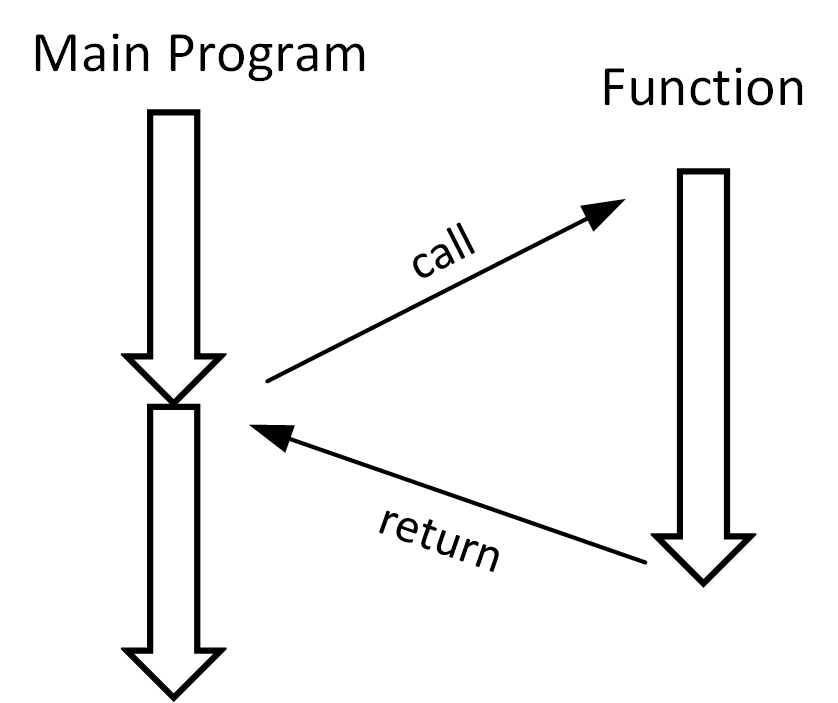
\includegraphics[width=.7\textwidth]{function}
\end{center}
\end{frame}

\begin{frame}[fragile]
  \frametitle{Functions}
\begin{itemize}
\item Extend set of built-in functions with opportunity for customization
\item Functions \textbf{can} consist of the following:
\begin{enumerate}
\item \emph{Name} to refer to (avoid existing function names in R)
\item \emph{Function body} is a sequence of statements
\item \emph{Arguments} define additional parameters passed to the function body
\item \emph{Return value} which can be used after executing the function
\end{enumerate}
\item Simple example
<<>>=
f <- function(x,y) {
  return(2*x + y^2)
}
f(-3, 5)
@
\end{itemize}
\end{frame}

\begin{frame}[fragile]
  \frametitle{Functions}
\begin{itemize}
\item General syntax
<<eval=FALSE>>=
functionname <- function(argument1, argument2, ...) { 
  function_body
  return(value)
}
@
\item \emph{Return value} is the last evaluated expression\\
$\rightarrow$ Alternative: set explicitly with \verb@return(...)@
\item Curly brackets can be omitted if the function contains only one statement (not recommended)
\item Be cautious since the \emph{order of the arguments matters}
\item Values in functions are \emph{not printed} in console\\
$\rightarrow$ Remedy is \verb@print(...)@
\end{itemize}
\end{frame}

\begin{frame}[fragile]
  \frametitle{Examples of Functions}
<<>>=
square <- function(x) x*x # last value is return value
square(10)
@
<<>>=
cubic <- function(x) {
  # Print value to screen from inside the function
  print(c("Value: ", x, " Cubic: ", x*x*x))
  # no return value
}
cubic(10)
@
\end{frame}

\begin{frame}[fragile]
  \frametitle{Examples of Functions}
<<>>=
hello <- function() { # no arguments
  print("world")
}
hello()
@
<<>>= 
my.mean <- function(x) {
  return (sum(x)/length(x))
}
my.mean(1:100)
@
\end{frame}

\begin{frame}[fragile]
  \frametitle{Scope in Functions}
\begin{itemize}
\item Variables created inside a function only exists within it $\rightarrow$ \emph{local}
\item They are thus inaccessible from outside of the function
\item \emph{Scope} denotes when the name binding of variable is valid
<<>>=
x <- "A"
g <- function(x) {
  x <- "B"
  return(x)
}
x <- "C"
@
\item What are the values?
<<function_scope,eval=FALSE>>=
g(x) # Return value of function x
x    # Value of x after function execution
@
\pause
\item Solution
<<,echo=FALSE>>=
<<function_scope>>
@
\end{itemize}
\end{frame}

% TODO: move to later part
\begin{frame}[fragile]
  \frametitle{Unevaluated Expressions}
\begin{itemize}
\item Expressions can store \emph{symbolic mathematical statements} for later modifications (e.\,g. symbolic derivatives)
\item Let's define an example via \verb@expression(...)@
<<>>=
f <- expression(x^3+3*y-y^3-3*x)
f
@
\item If \emph{evaluation} of certain parameters becomes necessary, one can use \verb@eval(...)@
<<>>=
x <- 2
y <- 3
eval(f)
@
\end{itemize}
\end{frame}

\begin{frame}[fragile]
  \frametitle{If-Else Conditions}
\begin{itemize}
\item \emph{Conditional execution} requires a condition to be met
\end{itemize}

\begin{center}
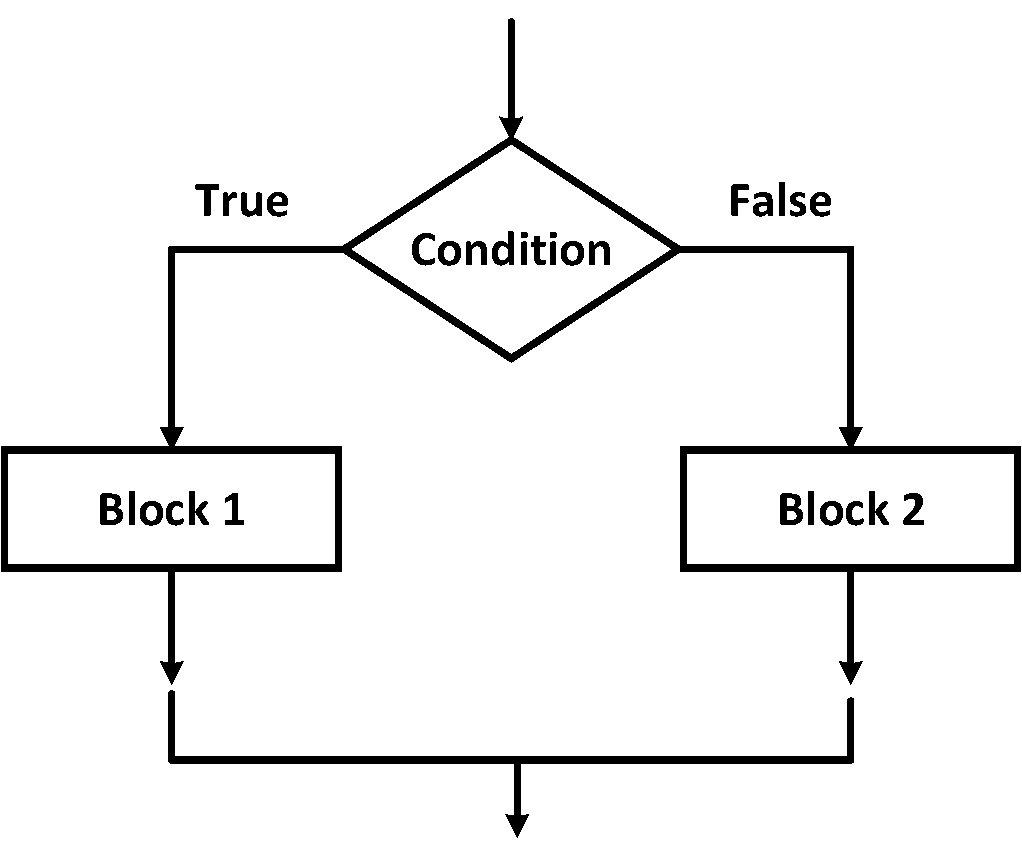
\includegraphics[width=.7\textwidth]{if-else}
\end{center}
\end{frame}

\begin{frame}[fragile]
  \frametitle{If-Else Conditions}
\begin{itemize}
\item Keyword \verb@if@ with optional \verb@else@ clause
\item General syntax:
\begin{columns}[T]
\begin{column}{.35\textwidth}
\textbf{if condition}\\
<<,eval=FALSE>>=
if (condition) {
  statement1
}
@
If \verb@condition@ is true, then \verb@statement@ is executed
\end{column}
\begin{column}{.4\textwidth}
\textbf{if-else condition}
<<,eval=FALSE>>=
if (condition) {
  statement1
} else {
  statement2
}
@
If \verb@condition@ is true, then \verb@statement1@ is executed, otherwise \verb@statement2@
\end{column}
\end{columns}	
\end{itemize}
\end{frame}

\begin{frame}[fragile]
  \frametitle{If-Else Conditions}
\begin{itemize}
\item Example
\begin{columns}[T]
\begin{column}{.35\textwidth}
<<>>=
grade <- 2
if (grade <= 4) {
  print("Passed")
} else {
  print("Failed")
}
@
\end{column}
\begin{column}{.35\textwidth}
<<>>=
grade <- 5
if (grade <= 4) {
  print("Passed")
} else {
  print("Failed")
}
@
\end{column}
\end{columns}	
\item Condition must be of length 1 and evaluate as either \verb@TRUE@ or \verb@FALSE@
<<>>=
if (c(TRUE, FALSE)) { # don't do this!
  print("something")
}
@
\end{itemize}
\end{frame}

\begin{frame}[fragile]
  \frametitle{Else-If Clauses}
\begin{itemize}
\item \emph{Multiple conditions} can be checked with \verb@else if@ clauses
\item The last \verb@else@ clause applies when no other conditions are fulfilled
\item The same behavior can also be achieved with \emph{nested if-clauses}
\begin{columns}[T]
\begin{column}{.4\textwidth}
\textbf{else-if clause}\\
<<,eval=FALSE,size='scriptsize'>>=
if (grade == 1) {
  print("very good")
} else if (grade == 2) {
  print("good")
} else {
  print("not a good grade")
}
@
\end{column}
\begin{column}{.4\textwidth}
\textbf{Nested if-condition}
<<,eval=FALSE,size='scriptsize'>>=
if (grade == 1) {
  print("very good")
} else {
  if (grade == 2) {
    print("good")
  } else {
    print("not a good grade")
  }
}
@
\end{column}
\end{columns}	
\end{itemize}
\end{frame}

\begin{frame}[fragile]
  \frametitle{If-Else Function}
\begin{itemize}
\item As an alternative, one can also reach the same control flow via the function \verb@ifelse(...)@ 
<<,eval=FALSE>>=
ifelse(condition, statement1, statement2) 
# executes statement1 if condition is true, 
# otherwise statement2
@
<<>>=
grade <- 2
ifelse(grade <= 4, "Passed", "Failed")
@
\item \verb@ifelse(...)@ can also work with vectors as if it was applied to each element separately
<<>>=
grades <- c(1, 2, 3, 4, 5)
ifelse(grades <= 4, "Passed", "Failed")
@
\item This allows for the efficient comparison of vectors
\end{itemize}
\end{frame}

\begin{frame}[fragile]
  \frametitle{For Loop}
\begin{itemize}
\item \verb@for@ loops execute statements for a \emph{fixed number of repetitions}
\end{itemize}

\begin{center}
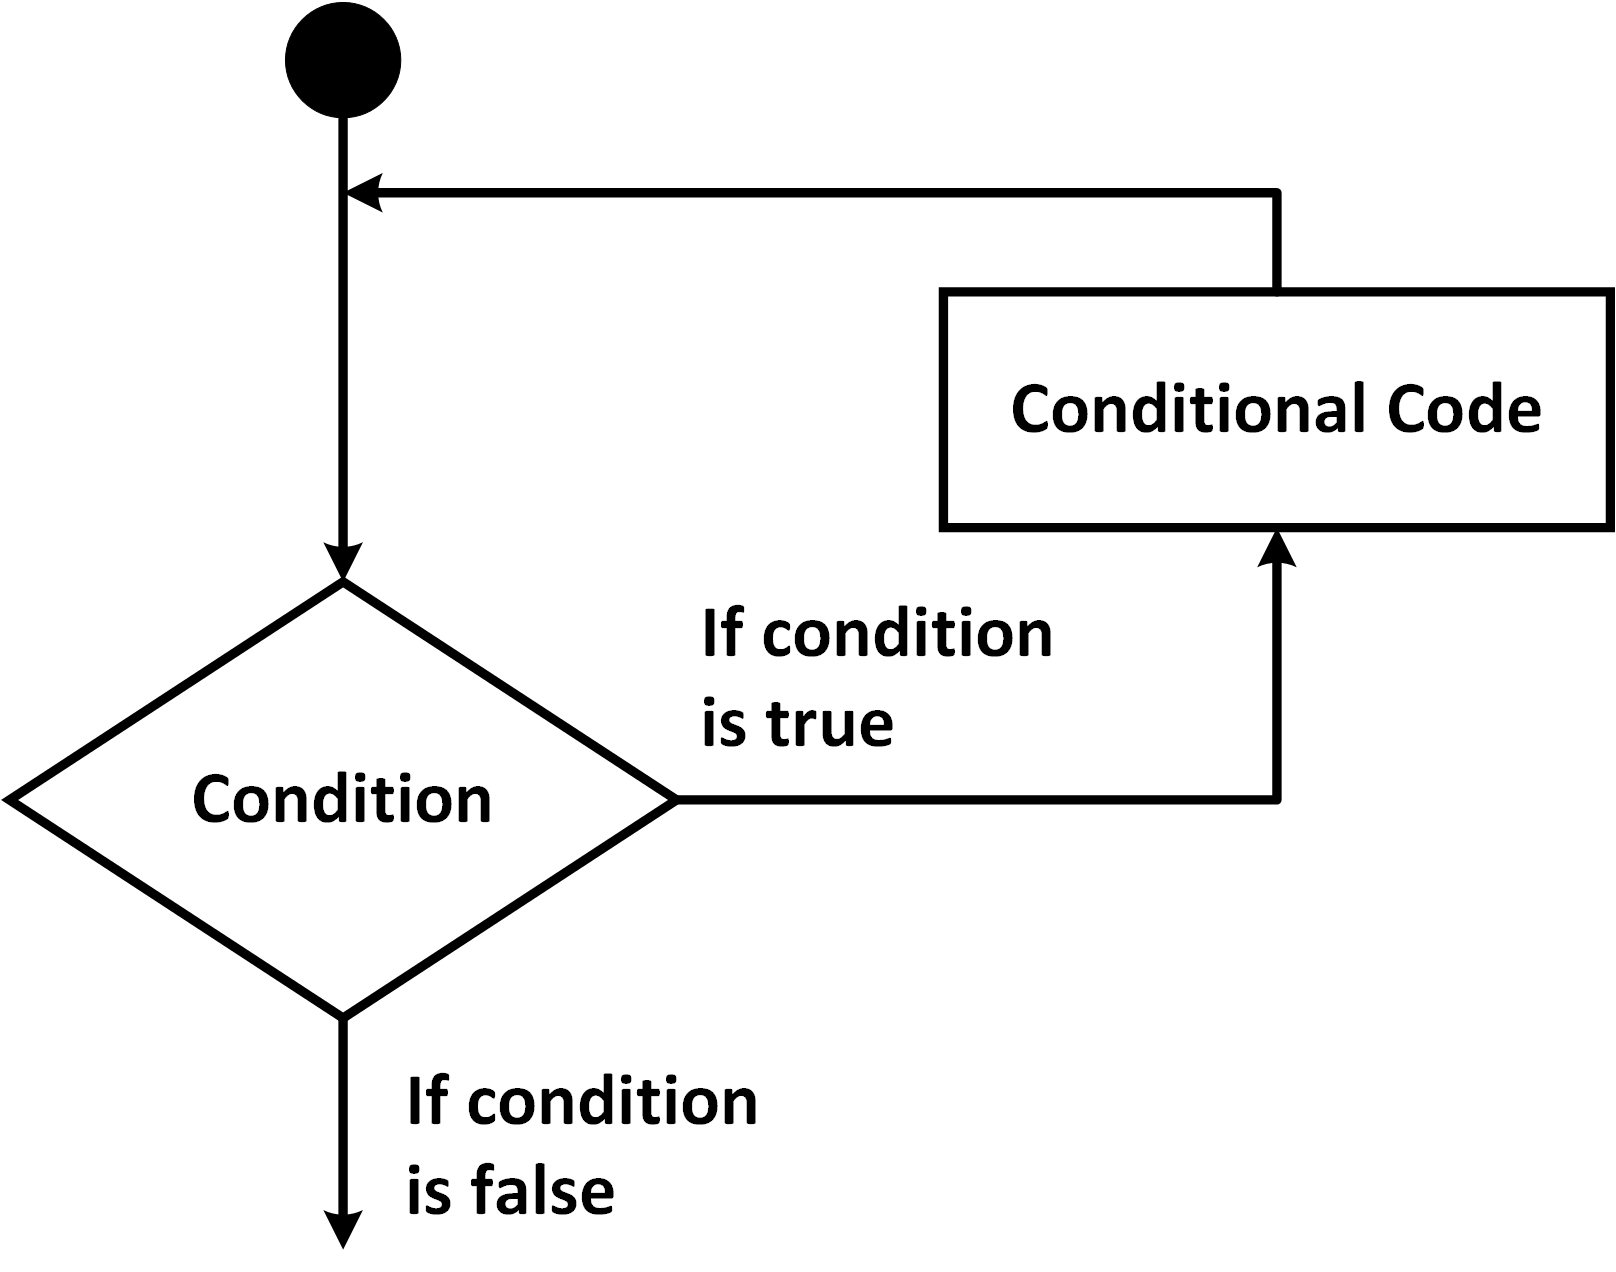
\includegraphics[width=.7\textwidth]{loop}
\end{center}
\end{frame}

\begin{frame}[fragile]
  \frametitle{For Loop}
\begin{itemize}
\item General syntax
<<eval=FALSE>>=
for (counter in looping_vector){
  # code to be executed for each element in the sequence
}
@
\item In every iteration of the loop, one value in the looping vector is assigned to the \verb@counter@ variable that can be used in the statements of the body of the loop. 
\item Examples
\begin{columns}[T]
\begin{column}{.3\textwidth}
<<eval=TRUE>>=
for (i in 4:7) {
  print(i)
}
@
\end{column}
\begin{column}{.5\textwidth}
<<eval=TRUE>>=
a <- c()
for (i in 1:3){
  a[i] <- sqrt(i)
}
a
@
\end{column}
\end{columns}	
\end{itemize}
\end{frame}

%\begin{frame}[fragile]
%  \frametitle{Foreach Loops}
%A shorter version of our above for loop is given through the function {\color{blue} foreach}. It additionally provides us with the possibility to run for loops on multiple processors/ cores parallely.
%<<>>=
%library(foreach)
%x <- foreach(i=1:3) %do% sqrt(i)
%x
%@
%\end{frame}

\begin{frame}[fragile]
  \frametitle{While Loop}
\begin{itemize}
\item \emph{Loop} where the number of iterations is \emph{controlled by a condition}
\item The condition is checked in every iteration
\item When the condition is met, the loop body in curly brackets is executed 
\item General syntax
<<eval=FALSE>>=
while (condition) {
  # code to be executed
}
@
\item Examples
\begin{columns}[T]
\begin{column}{.4\textwidth}
<<,size='scriptsize'>>= 
z <- 1
# same behavior as for loop
while (z <= 4) { 
    print(z)  
    z <- z + 1
}
@
\end{column}
\begin{column}{.4\textwidth}
<<,size='scriptsize'>>= 
z <- 1
# iterates all odd numbers
while (z <= 5) { 
    z <- z + 2
    print(z)  
}
@
\end{column}
\end{columns}
\end{itemize}
\end{frame}

\section{Timing}

%% http://www.ats.ucla.edu/stat/r/faq/timing_code.htm

\begin{frame}[fragile]
  \frametitle{Measuring Timings via Stopwatch}
\begin{itemize}
\item \emph{Efficiency} is a major issue with larger datasets and complex codes
\item Timings can help in understanding scalability and bottlenecks 
\item Use a stopwatch approach measuring the duration between two \verb@proc.time()@ calls
\end{itemize}	
<<,size='scriptsize'>>=  
start.time <- proc.time() # Start the clock

g <- rnorm(100000)
h <- rep(NA, 100000)
for (i in 1:100000) { # Loop over vector, always add +1
  h[i] <- g[i] + 1
}

# Stop clock and measure duration
duration <- proc.time() - start.time
@
\end{frame}

\begin{frame}[fragile]
  \frametitle{Measuring Timings via Stopwatch}
\begin{itemize}
\item Results of \verb@duration@ have the following format
<<,echo=FALSE>>=
duration
@
\item Timings are generally grouped into 3 categories
\begin{itemize}
\item \emph{User} time measures the understanding of the R instructions
\item \emph{System} time measures the underlying execution time
\item \emph{Elapsed} is the difference since starting the stopwatch ($=$ user $+$ system)
\end{itemize}
\item Alternative approach avoiding loop
<<>>=
start.time <- proc.time() # Start clock
g <- rnorm(100000)
h <- g + 1
proc.time() - start.time # Stop clock
@
\item Rule: \emph{vector operations are faster} than loops
\end{itemize}	
\end{frame}

\begin{frame}[fragile]
   \frametitle{Measuring Timings of Function Calls}
Function \verb@system.time(...)@ can directly time function calls
<<>>=
slowloop <- function(v){ 
	for (i in v) {
	  tmp <- sqrt(i)
	}
}

system.time(slowloop(1:1000000)) 
@
\end{frame}

\section{Wrap-Up}

\begin{frame}[fragile]
  \frametitle{Fancy Diagrams with ggplot2}
<<ggplot2,eval=FALSE,size='tiny'>>=
library(ggplot2)
@%
<<,include=FALSE>>=
<<ggplot2>>
@%
\vspace*{-0.5cm}
<<ggplot2_plant,tidy=FALSE,size='tiny'>>=
df <- data.frame(Plant=c("Plant1", "Plant1", "Plant1", "Plant2", "Plant2", "Plant2"), 
                 Type=c(1, 2, 3, 1, 2, 3), 
                 Axis1=c(0.2, -0.4, 0.8, -0.2, -0.7, 0.1), 
                 Axis2=c(0.5, 0.3, -0.1, -0.3, -0.1, -0.8))
ggplot(df, aes(x=Axis1, y=Axis2, shape=Plant, 
               color=Type)) + geom_point(size=5)
@
\end{frame}

\begin{frame}[fragile]
  \frametitle{Summary: Visualization and Timing}
\vfill
%\begin{block}{}
{\renewcommand{\arraystretch}{1.2}%
\begin{tabular}{ll}
\verb@plot()@ & Simple plot function \tabularnewline
\verb@text()@ & Add text to an existing plot \tabularnewline
\verb@outer()@ & Apply a function to two arrays \tabularnewline
\verb@persp()@ & Plot a surface in 3D \tabularnewline
\verb@image()@ & Plot a colored image \tabularnewline
\verb@contour()@ & Add contour lines to a plot \tabularnewline
\verb@trans3d()@ & Add point to an existing 3D plot \tabularnewline
\verb@points()@ & Add points to a plot \tabularnewline
\verb@proc.time()@ & Stopwatch for measuring execution time\tabularnewline
\verb@system.time(expr)@ & Measures execution time of an expression \tabularnewline
\end{tabular}
}
%\end{block}
\vfill
\end{frame}

\begin{frame}[fragile]
  \frametitle{Summary: Programming}
\vfill
%\begin{block}{}
{\renewcommand{\arraystretch}{1.2}%
\begin{tabular}{ll}
\verb@function(){}@ & Self-defined function \tabularnewline
\verb@expression()@ & Function with arguments not evaluated \tabularnewline
\verb@eval()@ & Evaluate an expression \tabularnewline
\verb@if@, \verb@else@  & Conditional statement \tabularnewline
\verb@for(){}@ & Loops over a fixed vector \tabularnewline
\verb@while@ & Loops while a condition is fulfilled \tabularnewline
\end{tabular}
}
%\end{block}
\vfill
\end{frame}

\begin{frame}
  \frametitle{Outlook}
\vfill
\begin{block}{Additional Materials}
\begin{itemize}
\item Further exercises in homework~2
\item Advanced materials beyond our scope
\begin{itemize}
\item Advanced R (CRC Press, 2014, by Wickham)\\
\url{http://adv-r.had.co.nz/}
\end{itemize}
\end{itemize}
\end{block}
\vfill
\begin{block}{Future Exercises}
R will be used to implement optimization algorithms
\end{block}
\vfill
\end{frame}

\end{document}

